\documentclass[11pt,a4paper]{report}

\usepackage[utf8]{inputenc}
\usepackage[francais]{babel}
\usepackage[T1]{fontenc}
\usepackage{amsmath}
\usepackage{amsfonts}
\usepackage{amssymb}
\usepackage{graphicx}
\usepackage[squaren,Gray]{SIunits}
\usepackage{numprint}
\usepackage{mhchem}


\author{Groupe 1246}
\title{Projet P3 LFSAB1503: Rapport de la première tâche}
\begin{document}
\maketitle

\section{Équation de la réaction et bilan de matière}

Il nous est demandé de rechercher la quantité des différents composés nécessaire à la synthèse de l'ammoniac.
Il nous était dit que l'ammoniac pouvait être obtenu à partir de dihydrogène ($H_2$) et de diazote ($N_2$).
Nous sommes donc arrivés à l'équation de synthèse de l'ammoniac suivante: 

$$N_2 + 3H_2 \rightarrow 2NH_3$$
 \ce{N_{2(g)} + 3H_{2(g)} -> 2NH_{3(g)}}

La masse molaire de l'ammoniac étant de \unit{17}{\gram\per\meter}, nous en avons déduit que une masse de \unit{1000}{\ton}
correspondait à \unit{\dfrac{10^{9}}{17}}{\mole}. Nous avons ensuite fait un tableau d'avancement de la réaction,
où les données sont exprimées en moles: 

\begin{figure}[h]
\begin{tabular}{|c|c|c|c|}
\hline 
 & $N_2$ & $3H_2 \Rightarrow$ & $2NH_3$ \\ 
\hline 
Initial & $\dfrac{10^{9}}{17}*\dfrac{1}{2}$ & $\dfrac{10^{9}}{17}*\dfrac{3}{2}$ & 0 \\ 
\hline 
Réaction & -$\dfrac{10^{9}}{17}*\dfrac{1}{2}$ & -$\dfrac{10^{9}}{17}*\dfrac{3}{2}$ & +$\dfrac{10^{9}}{17}$ \\ 
\hline 
Final & 0 & 0 & $\dfrac{10^{9}}{17}$ \\ 
\hline 
\end{tabular} 
\end{figure}

La réaction se produisant en continu, on peut calculer des flux de quantité pour une période de 24 heures.
On obtient selon nos calculs:

\begin{itemize}
  \item{une consommation de $N_2$ égale à: $\dfrac{\dfrac{10^{9}}{17}*\dfrac{1}{2}}{3600*24} \cong 340.41 $ \unit{}{\mole\per\second}.}
  \item{une consommation de $H_2$ égale à: $\dfrac{\dfrac{10^{9}}{17}*\dfrac{3}{2}}{3600*24} \cong 1021.241 $\unit{}{\mole\per\second}
  \item{une production de $NH_3$ égale à: $\dfrac{\dfrac{10^{9}}{17}}{3600*24} \cong 680.827$ \unit{}{\mole\per\second}
}}\end{itemize}

\section{Aspect thermique}
Selon nos recherches, nous avons trouvé que la réaction était exothermique ($\Delta H_{react} = -92.2kJ$).
Il nous était indiqué que la température du réacteur devait être maintenue à 500 degrés Celsius et que celui-ci, 
vu le caractère exothermique de la récation, pouvait être refroidi par un débit continu d'eau, dont la température 
variait entre 25 et 90 degrés Celsius.

\subsection{Calcul de volume d'eau nécessaire (pour une mole produite)}
Nous savons donc que: $$\Delta H_{react} = -92.2kJ$$
Nous savons aussi que:
 $$q = m*C*dT$$
où $C$ est la constante calorifique massique de l'eau valant \unit{4.18}{\joule\per\celsius.\gram} et m est 
 la masse totale du volume d'eau.

 Vu les indications données, on peut facilement trouver que $dT=65$. En supposant que la température initiale de 
 réacteur est de 500 degrés Celsius, il vient: 
$92200 = 4.18*65*m \Rightarrow \dfrac{92200}{4.18*65} = m = \unit{339.344}{\gram}, qui correspond à \unit{0.339344}{\liters} d'eau.

\subsection{Calcul du débit d'eau nécessaire}

Nous avions calculé plus haut que le rythme de production de $NH_3$ était de environ \unit{680.827}{\mole\per\second},
il vient donc:  $680.827*0.339344 = 231.03$. 
le débit d'eau nécessaire serait donc de \unit{231.03}{\liter\per\second}.

\begin{figure}[ht!]
 \centering
 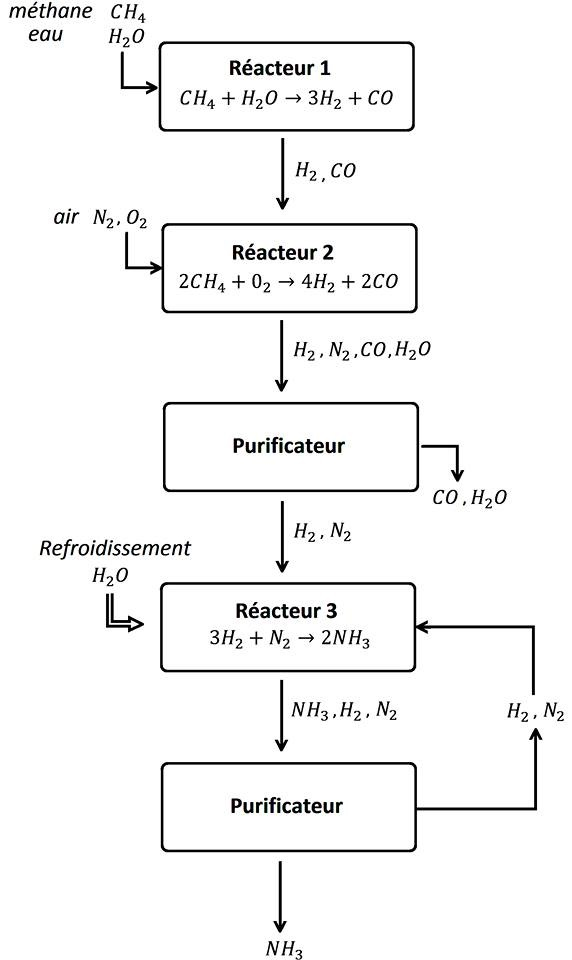
\includegraphics[scale=0.6]{flowsheet.jpg}
 \caption{Schéma}
 \label{scheme}
 
\end{figure}

\end{document}
